\documentclass{sig-alternate}

\usepackage[draft,nomargin,footnote]{fixme}

\usepackage{xspace}
\newcommand{\eg}{\textit{e.g.}\xspace}
\newcommand{\etal}{\textit{et al.}\xspace}
\newcommand{\ie}{\textit{i.e.}\xspace}
\newcommand{\etc}{\textit{etc.}\xspace}
\newcommand{\vs}{\textit{vs.}\xspace}

\graphicspath{{figs/}}

\begin{document}
%
% --- Author Metadata here ---
\conferenceinfo{HRI}{'16 Chrischurch, New Zealand.}
%\CopyrightYear{2007} % Allows default copyright year (20XX) to be over-ridden - IF NEED BE.
%\crdata{0-12345-67-8/90/01}  % Allows default copyright data (0-89791-88-6/97/05) to be over-ridden - IF NEED BE.
% --- End of Author Metadata ---

\title{Real-time Attention Assessment for Social Robots}
\author{Fernando Garcia \qquad Séverin Lemaignan \qquad Alexis Jacq \qquad Pierre Dillenbourg\\Computer-Human Interaction in Learning and Instruction Laboratory (CHILI)\\École Polytechnique Fédérale de Lausanne (EPFL)}


\maketitle
\begin{abstract}
Successfully sustaining face-to-face interaction between humans and robots mandates fine perception of each other attentional focus. Along this line, we present a novel technique to assess the visual focus of attention (VFOA) based on accurate, real-time head pose estimation with monocular camera. The software is fully open-source and can readily be adopted on a wide range of social robots. We propose an in-depth evaluation of the technique, using manual video annotations as ground truth, and show that our system reaches high level of accuracy in a real-world face-to-face interaction scenario. We finally show how to derive a metric of engagement from the monitoring of the VFOA, allowing the robot to account and react to the user's changing engagement in real-time.
\end{abstract}

%% A category with the (minimum) three required fields
%\category{H.4}{Information Systems Applications}{Miscellaneous}
%%A category including the fourth, optional field follows...
%\category{D.2.8}{Software Engineering}{Metrics}[complexity measures, performance measures]

\terms{Experimentation, Human Factors.}

\keywords{Human-Robot Interaction; Social Robotics; Attention Assessment; Engagement; Computer Vision.}

\section{Introduction}

In the recent years, research is pushing forward in building intelligent systems and environments that try to maximize the benefits of cooperation with humans based on verbal and non-verbal communication. The interaction between social robots and humans entails a broad set of situations, and evidences the need for capturing significant backchannel information generated by the user during the interaction process. Such information is used to adapt the system to the specific user's needs to eventually provide a social or emotional intelligence to the agents.

It is indeed not enough to exhibit human-like capabilities in social tasks: a robot needs to achieve human-like manners. For instance, several studies showed that humans prefer to interact with robots whose task outcome is delayed, shows uncertainty or an undesired output \cite{Admoni,Short}. In fact, the ability to adapt has been proved to be beneficial in long-term interactions \cite{Tielman:2014, Lim:2014}, specifically with children, manifesting a more positive attitude over time.

In order to build intelligent agents, it is necessary to equip them with a range of perceptual capabilities: while face and object tracking and recognition~\cite{Zhao:2003, Jafri:2014}, path planning~\cite{Galceran:2013}, speech recognition~\cite{brick2007incremental} or task learning~\cite{calinon2007learning} are amongst the current major research directions, existing literature tends to evaluate each of these algorithms in their own metric space, without considering the overall interaction quality. Along this line, Anzalone \etal~\cite{anzalone} have recently argued in favor of such a global evaluation, and propose to assess these algorithms in term of their capability to obtain the desired effect in a human-robot interaction context, and they correspondingly propose metrics build around the measurement of \emph{engagement} as indicator of the quality of the experience.

Engagement describes a cognitive, affective (specifically intrinsic motivation), and behavioral state of interaction with a computer application that ``makes the user want to be there" \cite{OBrien:2010}. Engaging interactions were thought to involve attention, intrinsic interest, interactivity, perceived control and choice, functionality and motivation.

In this way, in situ Visual Focus of Attention (VFOA) estimation is advantageous to human-robot interaction and a major contribution towards a better understanding of the interaction quality.\cite{yarbus1967eye, barber1976perception} suggest that human's interest is highly correlated with what they look at and the existing relationship between gaze and attention during social interaction has been exposed in~\cite{argyle1969social}.\fxfatal{This paragraph is not well connected to the previous ones}

\subsection{Importance in learning environments}

Education and learning environments are interesting application fields for research on attention assessment, since sustaining children's engagement over time is a key variable to ensure
effective learning (see for instance~\cite{Umbach}), and they indeed motivate this research. Besides, while~\cite{zhao2012learning} recommends the development of a teachable agent that is actively, rather than passively, engaged in the learning by teaching interaction, the increased learning gain results attained in~\cite{okita2006observation} were done so even with the pupil being taught having been instructed to not contribute much information. This suggests that it may not be necessary, from a learning by teaching point of view, for the teachable agent to participate actively in the interaction to incite educational benefits. However, from an engagement point of view, this may not necessarily be true.\fxfatal{rephrase, and be careful: 'learning by teaching' is only introduced in the next paragraph}

In fact, the use of robots in education comes with the potential to engage the child in meta-cognition through the learning by teaching paradigm, wherein a student takes the role of a teacher and experiences stronger educational benefits as a result (such as in \cite{Palinscar1984}).\fxnote{to be merged with previous paragraph?}

The goal of this research is therefore to \textbf{evaluate the quality of an interaction} using the \textbf{visual focus of attention as an engagement indicator}. We validate our approach with field experiments conducted in the educational context of the CoWriter project~\cite{Hood:2015}, where our technique, being based on a regular, low-end RGB camera, avoids the use of otherwise typically invasive technologies such as eyetrackers, that would negatively impact the natural of the interaction.

\subsection{Related Work}

The notion of engagement has actively been studied in a diverse set of domains, and several variables and social signals have been proposed in the literature to quantify and study it in social interactions.

The evaluation of response times to provide an estimation of the user's engagement based on the correctness has been proposed in a learning context \cite{Beck} before. However, several aspects like the inter-subject variability or the environment complexity make it hardly applicable in a child-robot interaction. Additionally, other techniques \cite{Chipman07postureas} like the use of the weight distribution using a pressure sensitive chair has reported results. But it is in the computer vision field where major contributions have been done. 

In \cite{peters2010investigating} approach, a model of user's interest and engagement with a virtual agent displaying shared attention behavior, by using eye gaze and head direction information is proposed. Similarly, in \cite{nakano2010estimating} an approach to estimate the user's conversational engagement with a conversational agent based on analysis of gaze patterns was implemented. Other significant work \cite{Castellano:2009} focus on feature evaluation related to the user's non-verbal behavior, the task and the companion's affective reactions are identified to predict the children's level of engagement using a Bayesian model.

Some few studies have proposed approaches for the detection of engagement with a robot. In \cite{Rich:2010} a computational model based on the recognition of connection events such
as directed gaze, mutual facial gaze is proposed. In this context, some other \cite{Sanghvi:2011} focus only on the back or trunk posture as a determined factor for the assessment. A recent study \cite{anzalone} with social robots in face to face scenarios proposed a set of metrics based on non-verbal cues but manifesting some possible limitations in long-term scenarios.

In this research, we address the problem of tracking the children's engagement based on their VFOA and current performed task during a long term child-robot interaction in a learning context, first. And second, we provide qualitative and quantitative evaluation of the outcome provided using a first person RGB sensor approach. Moreover, this monitoring activity has been supporting our research in child-robot interaction for learning and instruction purposes.
\vfill


\subsection{Research Questions}

The participants' VFOA acquisition is the only dependent variable. This includes their gaze times and patterns of looking or not looking to the targets and the synchrony on the movements. This data extracted from an RGB camera was also coded post-hoc to quantify some of these measurements.

We predict that there will be no generalizable pattern of participant's VFOA behavior for different scenarios such as multiple subjects, necessitating in situ VFOA estimation capabilities to enable robots to adapt in the specific scenarios. However, we believe that off-line pattern identification can lead to a better understanding of the children progression as well as engagement level assessment in face-to-face long term interactions.

\section{Approach}

We propose a adaptive model based solution to approach head pose estimation that finds correspondences between facial landmarks points and their respective locations in a face model. We use the open-source library dlib\footnote{http://dlib.net} \cite{dlib09}, to detect and extract the skeleton of the subject's face and then, use the obtained landmarkers to calculate the head pose orientation estimation (see figure \ref{system}). In this way, we can estimate what the subject was looking at and obtain an \textit{rviz} 3D scene representation as it is executed as a ROS (Robot Operating System) node that can be seen in figure \ref{rviz}. Compared to intrusive hardware like head mounted displays, eye-trackers or wearables for instance, this approach has a clear advantage of simplicity and integration with robotic systems, but also becomes accurate enough for general purposes in face-to-face interactions. In addition, it allows us to model complex environments, handling different number and positions of participants in the scene.

\begin{figure}[h!]
    \centering
    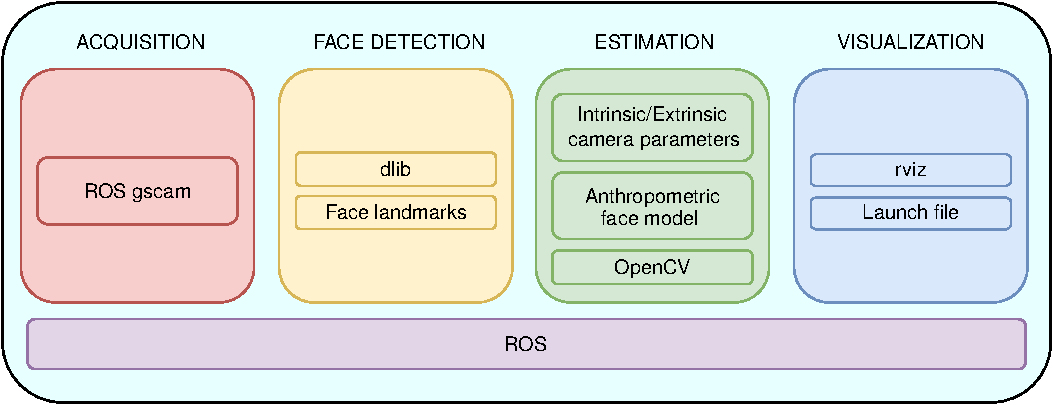
\includegraphics[width=0.9\columnwidth]{system}
    \caption{\small System overview showing the most relevant components involved in the estimation.}
    \label{system}
\end{figure}


\begin{figure}
    \centering
    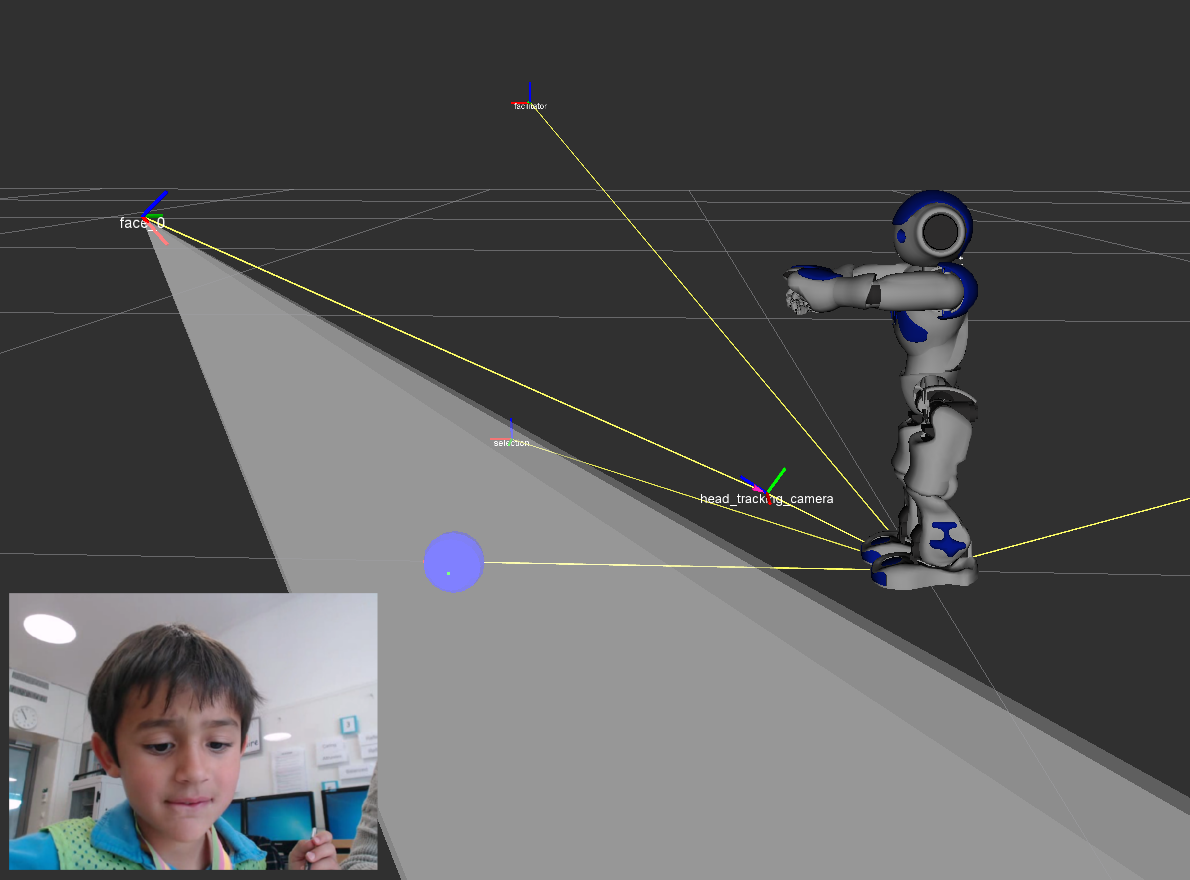
\includegraphics[width=0.9\columnwidth]{rviz_camera}
    \caption{\small Rviz screenshot showing Nao, camera (Nao's feet), face detected with its field of view (gray cone) and blue marker intersecting as current VFOA.}
    \label{rviz}
\end{figure}

\subsection{Estimating Head Pose}
The first step is to estimate the head pose using the pin-hole model shown in equation \ref{eq:pinHole}. As mentioned above, dlib library facilitates the task by providing the 2D points \textit{m'} that composes the face silhouette. However, it is enough with obtaining eight spread points, such as right and left eyes, right and left tragions, sellion or nasal depression zone, pronasale or center of the nose, stomion or center of the mouth and menton.

Likewise, the 3D face model is needed. The proposed head pose estimation method would work best with a 3D face model of the query subject itself. When a 3D face model of the subject is not available, as in many practical situations, a generic 3D face model can be used. This is an estimation of the same anthropometric points \textit{M'} (for North American Caucasians) in the 3D space \cite{farkas1994anthropometry}. Moreover, the intrinsic camera parameters are necessary to be able to compose its matrix \textit{A}. The components are expanded in equation \ref{eq:pinHole2}.	

\begin{equation}
s  \; m' = A [R|t] M'
\label{eq:pinHole}
\end{equation}
\begin{equation}
s
\begin{bmatrix}
x \\
y \\
1
\end{bmatrix}
=
\begin{bmatrix}
f_x & 0 & c_x  \\
0 & f_y & c_y  \\
0 & 0 & 1 
\end{bmatrix}
\begin{bmatrix}
r_{11} & r_{12} & r_{13} & t_x  \\
r_{21} & r_{22} & r_{23} & t_y  \\
r_{31} & r_{32} & r_{33} & t_z  
\end{bmatrix}
\begin{bmatrix}
X \\
Y \\
Z \\
1
\end{bmatrix}
\label{eq:pinHole2}
\end{equation}

Finally, the matrix of extrinsic parameters [R|t] is obtained by joining the rotation matrix R (calculated from the rotation vector) and translation vector \textit{t}. The result is a matrix projection \textbf{P} which maps a point in the 3D space onto a point in the 2D image plane solving equation \ref{eq:p}.

\begin{equation}
s  \; m' = P \; M'
\label{eq:p}
\end{equation}

\subsection{Setting the \textit{tf} Frame}
The second step is to use the matrix [R|t] to set the correct translation and orientation of the \textit{tf} frame which represents the face in the 3D space. In order to achieve that it is necessary first, to set the origin defined by the vector \textit{t}. Second, the matrix \textit{R} needs to be reformulated into a quaternion as shown in equation \ref{eq:quat} due to the smoothly interpolation between them.

\begin{equation}
\begin{bmatrix}
qw \\
qx \\
qy \\
qz
\end{bmatrix}
=
\begin{bmatrix}
\sqrt{1 + r_{11} + r_{22} + r_{33}} /2 \\
(r_{32} - r_{23})/( 4 \cdot qw) \\
(r_{13} - r_{31})/( 4 \cdot qw) \\
(r_{21} - r_{12})/( 4 \cdot qw)
\end{bmatrix}
\label{eq:quat}
\end{equation}
\\
However, it is necessary to consider the cases where the division is performed by 0 (in 180\degree rotation about the y-axis for instance) or when \textit{qw} becomes close to zero.

\subsection{Defining the Field of View}
The third step is to generate a representation of the field of view whose origin and orientation are the ones defined by the face detection \textit{tf} frame. 

Defining accurately the human field of view in the implementation is a must. Holmqvist in \cite{holmqvist2011eye} specifies that the visual human range is $ \pm  40\degree $ in the horizontal and $ \pm 25\degree $ in the vertical. In \cite{walker1980clinical} Spector provides a more detailed specification for each eye splitting the vertical range into $ 60\degree $ the upper region and $ 75\degree $ the lower one. Moreover, the horizontal range gets separated in $ 60\degree $ inwards (towards the nose) and $ 95\degree $ outwards. In the present implementation, the first approach explained has been chosen representing the field of view using a cone with such dimensions.

Assuming that the \textit{tf} frames representing the robotic agent and the VFOA candidates are static, need to be monitored. This task consists on evaluating the intersection between the \textit{tf} frames and the field of view: If one focus of attention is within the region defined by the field of view, we assume the subject is looking at it. In order to solve such operation mathematically it is necessary to compute the transformation matrix between the coordinate frames to be able to locate the monitored frames \textit{A} in the subject's coordinate system \textit{B} (see equation \ref{eq:transform}).

\begin{equation}
v' = B(A^{-1})v
\label{eq:transform}
\end{equation}

where \textit{v} is a point in \textit{A} that becomes v' in coordinate system \textit{B}. However, in practice there are, at least, three different \textit{tf} frames involved in the transformation (subject-camera, camera-base, base-focus). Following the transformation result, the distance of the monitored frame with respect to the x-axis face \textit{tf} frame, $ d_{x_{axis}} $, representing the subject's face can be computed as simple as in equation \ref{eq:pitagoras}. Always considering the x-axis as the one defining the face's orientation and thus field of view's main axis.

\begin{equation}
d_{x_{axis}} = \sqrt{t_y^2 + t_z^2}
\label{eq:pitagoras}
\end{equation}

It is necessary to compare the distance acquired $ d_{x_{axis}} $ with the radius of the field of view at the target \textit{tf} frame x-coordinate $ r_{fov} $ as shown in equation \ref{eq:fovtf}.

\begin{equation}
r_{fov} = tan\left(\frac{fov}{2}\right) \cdot t_x
\label{eq:fovtf}
\end{equation}

where \textit{fov} is the aperture angle of the field of view. Finally, if $ d_{x_{axis}}<r_{fov} $, the target is within the subject's field of view.

% Schema to clarify this?

\section{Case Study}
The presented method have been successfully employed in a real child-robot interaction situation where the robot tries to engage the child in handwriting tasks using learning by teaching paradigm.
\subsection{Experimental Set-up}

The target of this study were 6 children with ages compressed between 5 and 6 years old. The experiments were developed individually and consisted on a writing activity by turns and one story telling performed by the robot at a given time of the interaction. All this performed in a over all 18 minutes interaction average time.

Figure~\ref{fig:realSetup} illustrates our general experimental setup: a
face-to-face child-robot interaction with an (autonomous) Aldebran's {\sc nao}
robot.

\begin{figure}[h!]
    \centering
    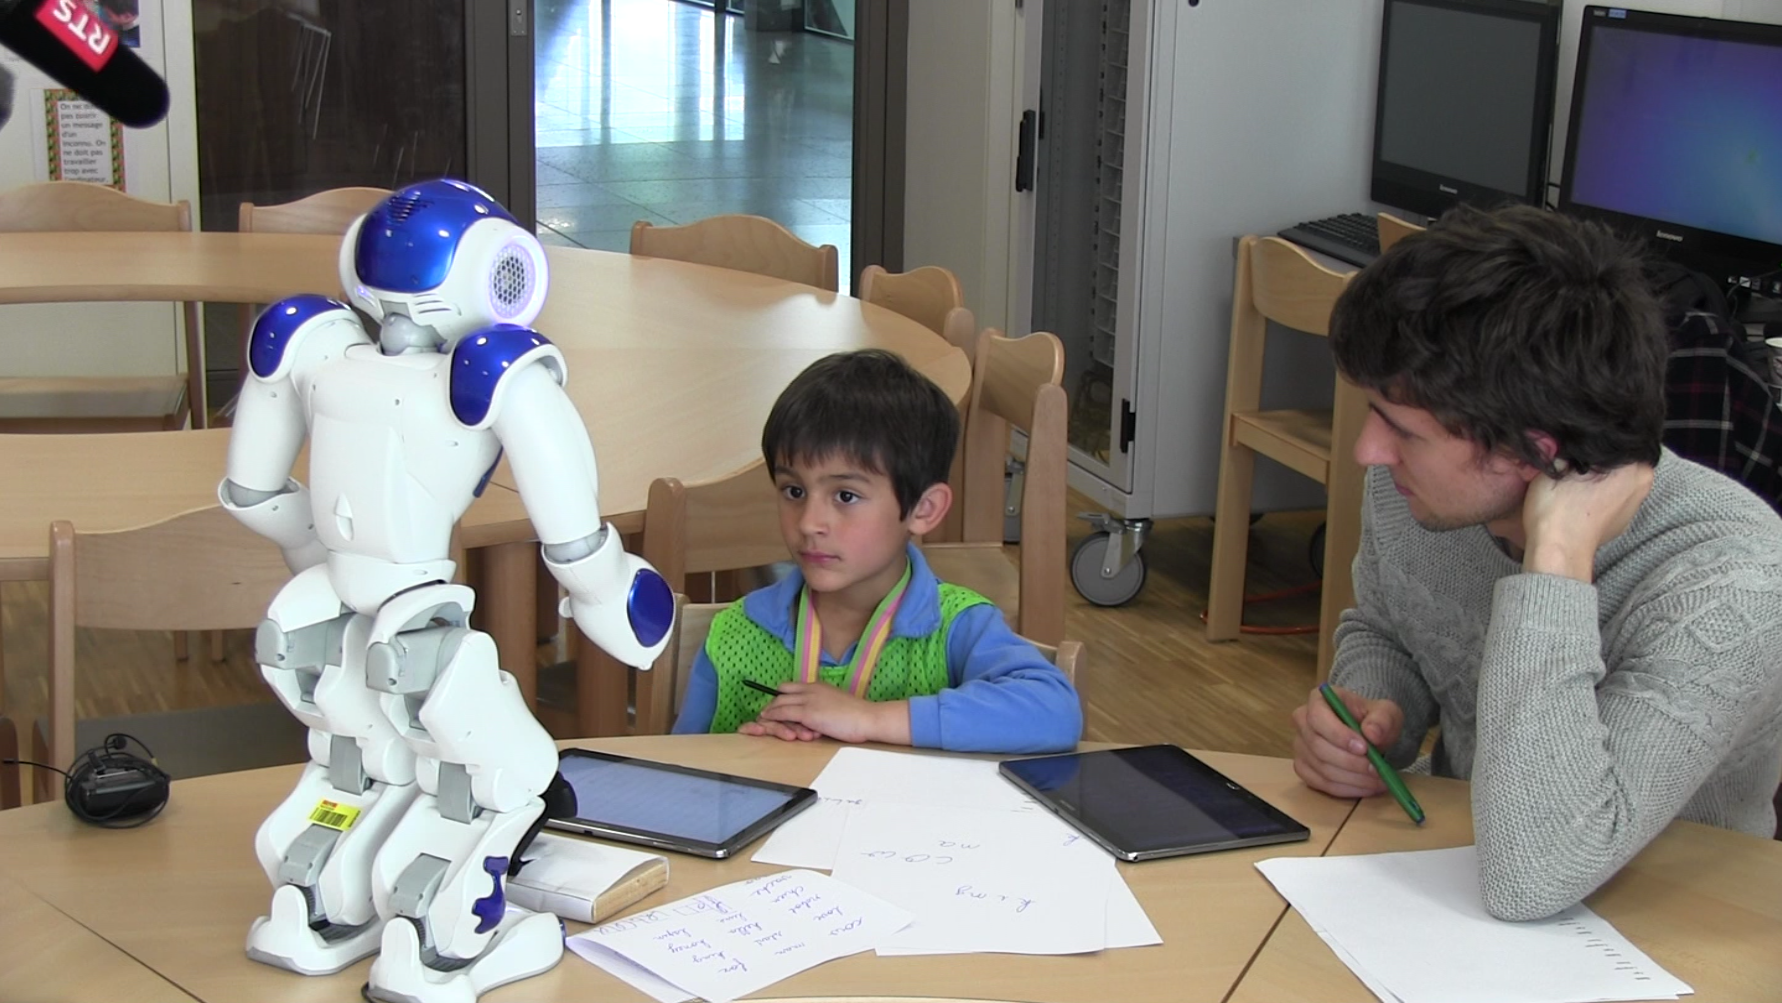
\includegraphics[width=1\columnwidth]{realSetup}
    \caption{\small Our experimental setup: face-to-face interaction with a {\sc
            nao} robot.  The robot writes on the tactile tablet, the child then
            corrects the robot by directly overwriting its letters on the tablet
            with a stylus. An adult (either a therapist or an experimenter,
            depending on the studies), remains next to the child to guide the work. 
            A second tablet allows to choose demonstrations and the camera captures the subject's face.}
    \label{fig:realSetup}
\end{figure}

A tactile tablet (with a custom application) is used for both the robot and the child to write: during a typical round, the child requests the robot to write something (a single letter, a number or a full word), and push the tablet towards the robot, the robot writes on the tablet by gesturing the writing (but without actually physically touching the tablet), the child then pull back the
tablet, corrects the robot's attempt by writing him/herself on top or next to the robot's writing, and ``send'' his/her demonstration to the robot by pressing a small button on the tablet. The robot ``learns'' from this demonstration and tries again.

Since the child is assumed to take on the role of the teacher, we had to ensure (s)he would be able to manage by him/herself the turn-taking and the overall progression of the activity (moving to the next letter or word). In our design, the turn-taking relies on the robot prompting for feedback once it is done with its writing (simple sentences like ``What do you think?''), and pressing on a
small robot icon on the tablet once the child has finished correcting. In our experiments, both were easy to grasp for children.

Implementing such a system raises several challenges that are discussed in detail in \cite{Hood:2015}.

An RGB camera has been used to acquire images of 640x480 pixels at 25 fps. The camera was located at 5 cm from the center of Nao's feet and its holder was tied to a wood base for stability purposes. Thus, the camera's objective was 9 cm above and $ 40\degree $ inclination with respect to the surface of the table to maximize the detection during the writing time. However, Nao's camera could have been used, always considering the \textit{tf} frame matrix update according to the head orientation.

The subjects were typically located 50 cm away from the robot with the first tablet in front and the second one 30 cm to the left of the first one. In the same way, the experimenter was located around 60 cm to the left of the subject. Finally, two observers were located far away from the interaction field to manually assess the state of the interaction.

Figure \ref{drawSetup} allows us to intuitively identify several focuses of attention along the interaction such as the two tablets, the robot, the experimenter and the observers located in the diagonal.

\begin{figure}[h!]
    \centering
    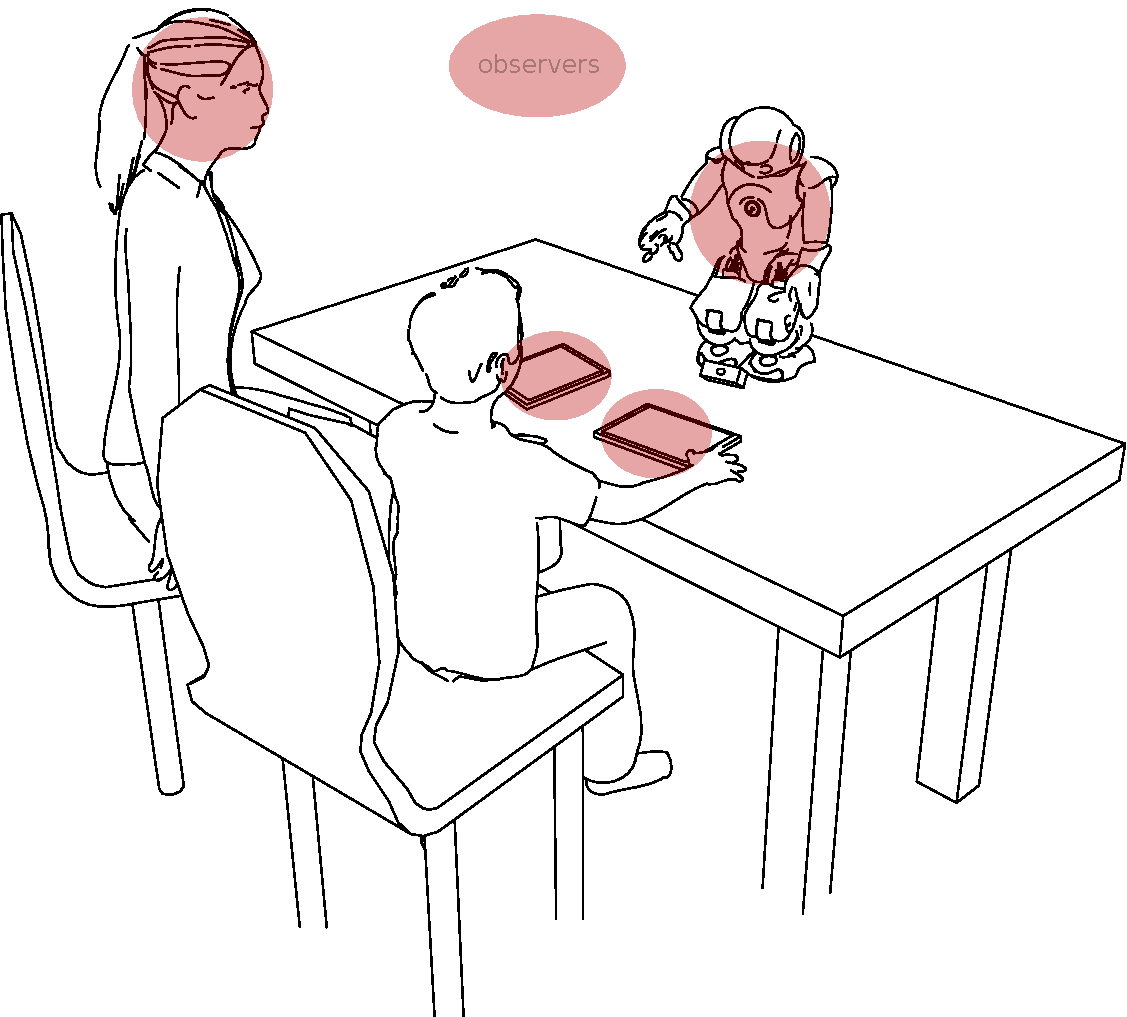
\includegraphics[width=0.7\columnwidth]{drawSetup}
    \caption{\small Graphical representation of the set-up and the possible children focuses of attention in the scene, in red.}
    \label{drawSetup}
\end{figure}


\section{Results}

In this work, head orientation is used to predict a person's focus of attention in face-to-face interactions. Therefore, we assume that head pose is a reliable marker of the attention focus during a social interaction, in both cases human-human, human-robot. Since we estimate where the subject is looking at based on its head position, several important questions arise:

\begin{enumerate}
\item Which head pose estimation tracking rate can we achieve during a real case scenario?  
\item How accurate can we predict where the subject is looking at based on the head pose estimation?
\item How can we evaluate the engagement of the children based on the focus of attention?\newline
\end{enumerate}

\subsection{From Face Detection to Focus of Attention} \label{fromFaceTo}

According to \cite{stiefelhagen2002tracking} the head orientation's contribution in overall gaze direction is 68.9\% showing agreement between both measurements. In addition, it shows that the head orientation alone can get an average accuracy of 88.7\% detecting the focus of attention in a meeting application scenario using a head-mounted display with eye and head tracking.

Our results for a peer-to-peer work scenarios using an approach based on RGB camera are summarized in table \ref{tab:results} where the \textit{expected} is the focus of attention that given the state of the system, it is likely to attract the subject's gaze. In the same manner, the \textit{captured} is the focus of attention our approach provides and the \textit{real}, the ground truth of the subject's gaze direction based on manual annotations from two evaluators with an average reliability of $ \alpha = .89 $.

In order to calculate the inter-rater reliability between the two measurements (real-captured and real-expected), the overlap percentage between the two curves has been computed. A more reliable measurement in terms of time shifting between the real and captured focuses of attention is provided using the cosine similarity also shown in table \ref{tab:results}. 

\begin{table}[h!]
	\centering
	\caption{Tracking accuracy in face-to-face scenario}
	\begin{tabular}{|c|c|c|c|c|c|c|c|} \hline
	\small Subject & 1 & 2 & 3 & 4 & 5 & 6 & Avg\\ \hline
	\small Track(\%) & \small88.2 & \small83.5 & \small90.5 & \small83.1 & \small87.9 & \small85.0 & \small86.4 \\ \hline
	\begin{tabular}{@{}c@{}}\small Real vs \\ \small expected(\%)\end{tabular} & \small92.6 & \small88.8  & \small95.8 & \small93.1 & \small96.5 & \small89.6 & \small92.7 \\ \hline
	\begin{tabular}{@{}c@{}}\small Real vs \\ \small captured(\%)\end{tabular} & \small61.1 & \small85.5 & \small80.8 & \small62.2 & \small63.4 & \small83.9 & \small72.8 \\ \hline
	\begin{tabular}{@{}c@{}}\small Cosine \\ \small affinity \end{tabular} & \small0.73 & \small0.82 & \small0.87 & \small0.73 & \small0.77 & \small0.89 & \small0.8 \\ \hline
	\end{tabular}
	\label{tab:results}
\end{table}

The results has proved that the VFOA prediction accuracy in the tracking is not only conditioned by the subject's amount of movement, but also by the speed of the same movements: Restless children externalize greater levels of movement decreasing the VFOA prediction accuracy. 

For instance, subjects 1,4 and 5 despite the fact that the tracking accuracy is in the average, the bad precision in the captured VFOA suggests that such children are highly likely to modify the gaze direction without head move intervention reducing dramatically the overlap between captured and real VFOA.

Additionally, several recurrent computer vision challenges such as the lighting conditions, occlusions with the hands and the face angle with respect to the camera, looking to the experimenter for instance, are factors that contribute to reduce the tracking accuracy.

\subsection{Subject's Focus of Attention Analysis}

\begin{figure*}
    \centering
    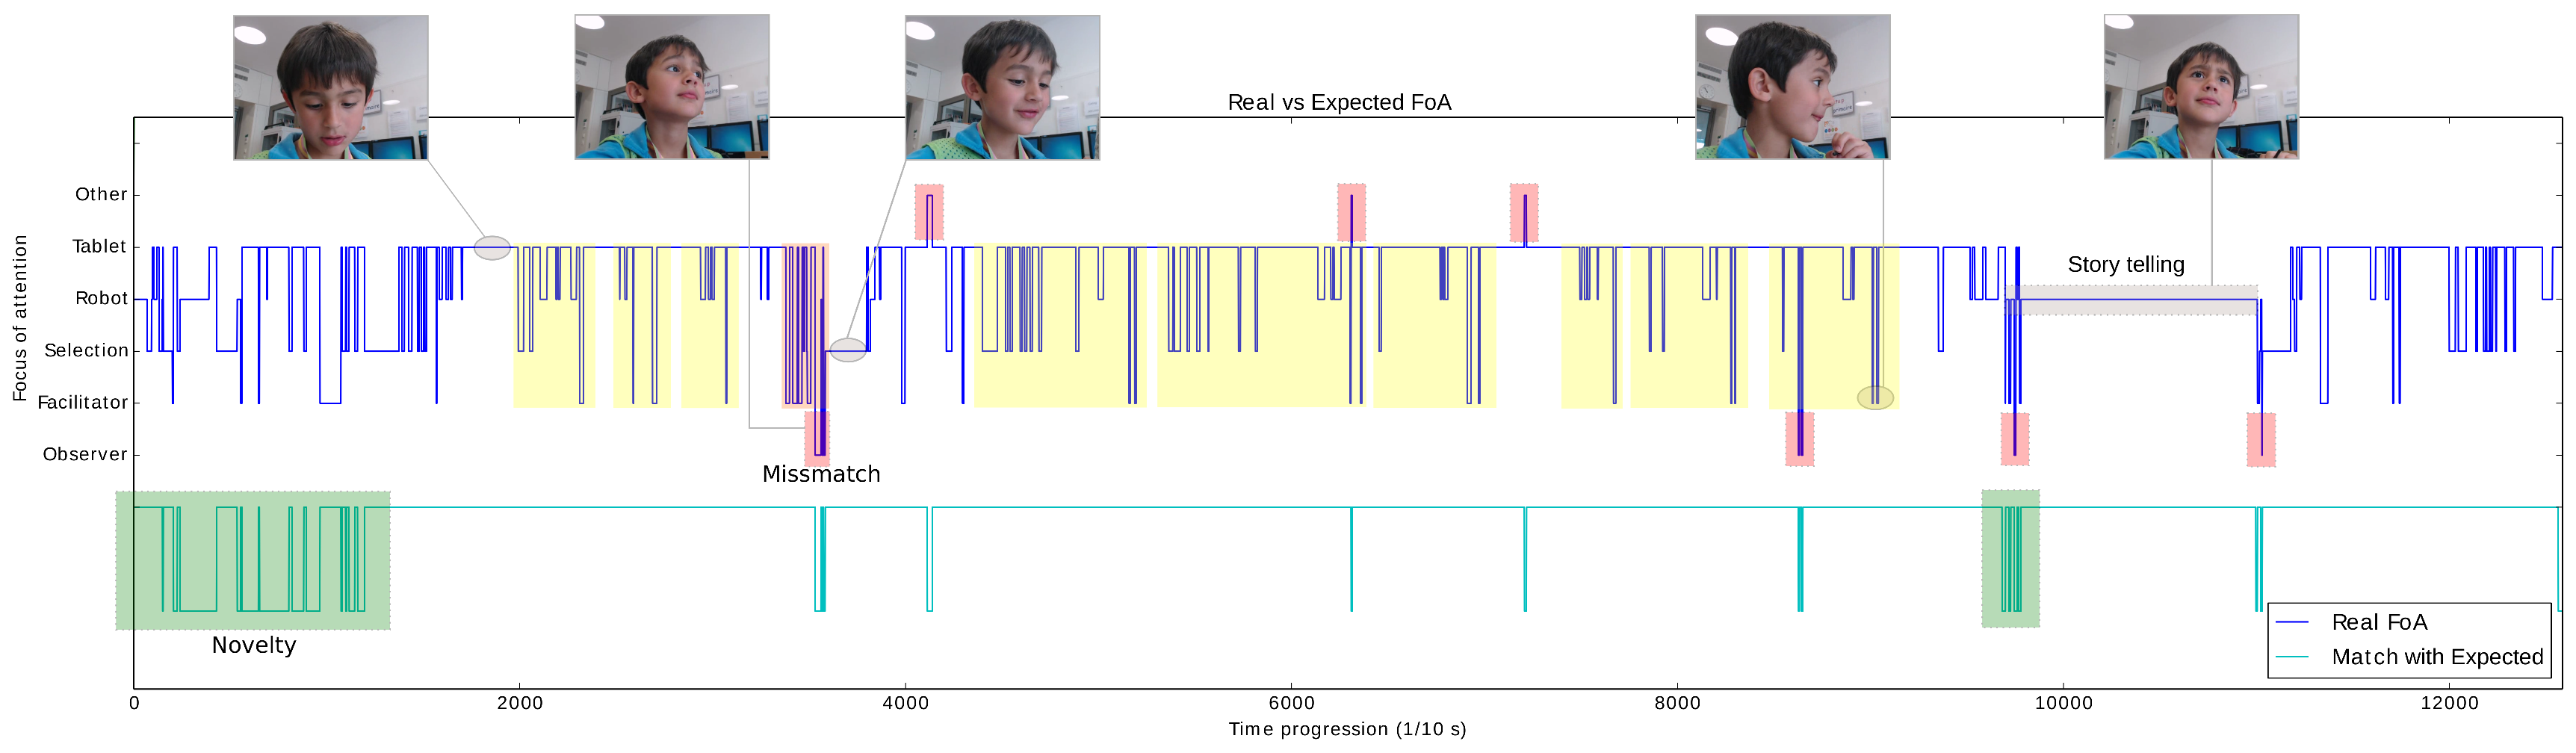
\includegraphics[width=1.8\columnwidth]{realExpected}
    \caption{\small In blue, real VFOA of subject 4 accoding to two observer's assessment. In cyan, the matching between the real and the obtained VFOA. In yellow, the repeated pattern in turn-taking and in orange, the experimenter's suggestion to choose a new word.}
    \label{fig:realExpected}
    
    % Maybe we should add the expected VFOA
\end{figure*}

\begin{figure*}
    \centering
    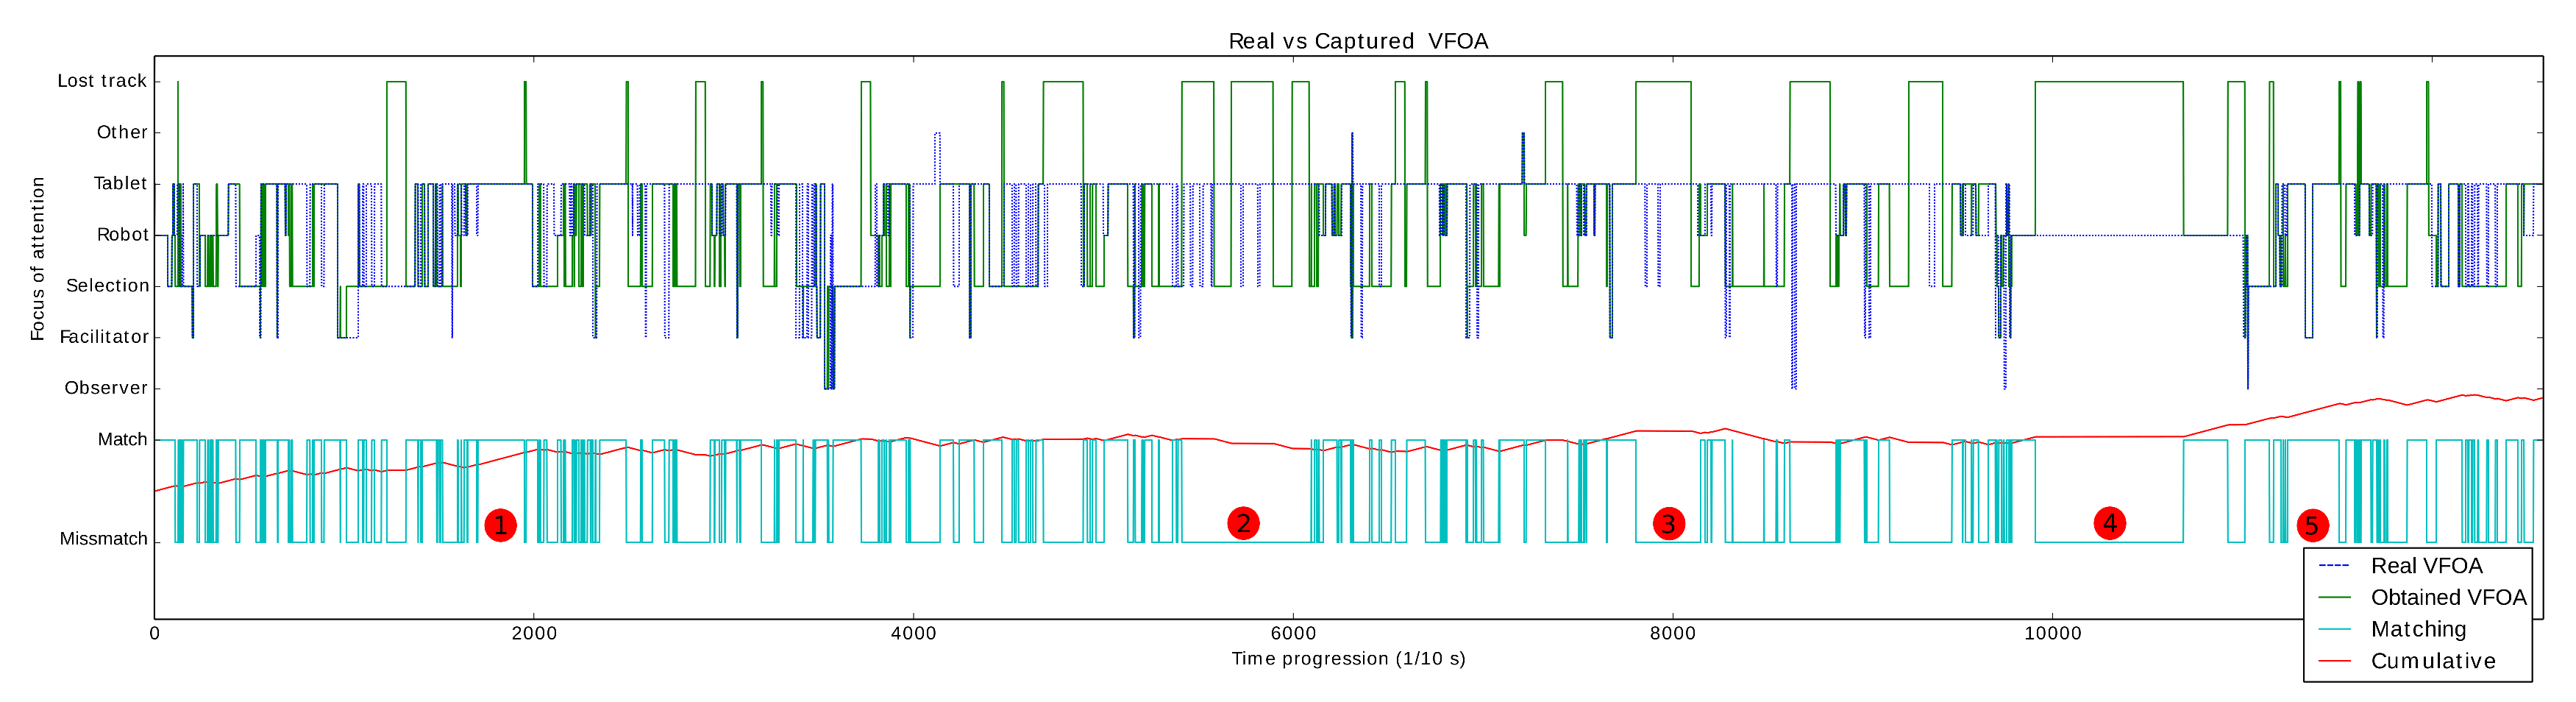
\includegraphics[width=1.81\columnwidth]{realCaptured}
    \caption{\small Real VFOA of subject 4 accoding to two observer's assessment. In green, the obtained VFOA using our aproach and in cyan, the mathing between them. Finally, the correspondent numbers with figure \ref{fig:bitmap}.}
    \label{fig:realCaptured}
\end{figure*}

According to figure \ref{fig:realExpected} several findings can be analyzed in detail. The matching curve (cyan color) shows the overlapping between the expected and the real focuses of attention. As can be noticed there is a fluctuation at the beginning of the interaction as well as just before the activity switching. These chaotic gaze manifestation is what we call an automatic discovery of events, when the user experiences an uncertainty in the present situation. 

The first one of the previous two situations presented above is due to the novelty effect the subjects experience for the first time in front of the system and according to the rest of participants suggests that the adaptation time is around the first 2 minutes of interaction. In the second case, an unexpected robot behavior produces such reaction due to an activity switching, the story telling.

It is important to consider that in some occasions during the interaction, none of the focuses of attention were within the field of view due to the time transition from one focus to another resulting in an ambiguity. In order to deal with these few cases it is assumed that the minimum distance between the height of the field of view (cone) and the targets corresponds to the most likely focus of attention. However, we also want to distinguish such cases when the subject is directly not looking where the defined targets are located, but towards a region far from the interaction field. These cases are not common but they can be easily identified by setting a horizontal threshold to the field of view.

\begin{figure}[h!]
    \centering
    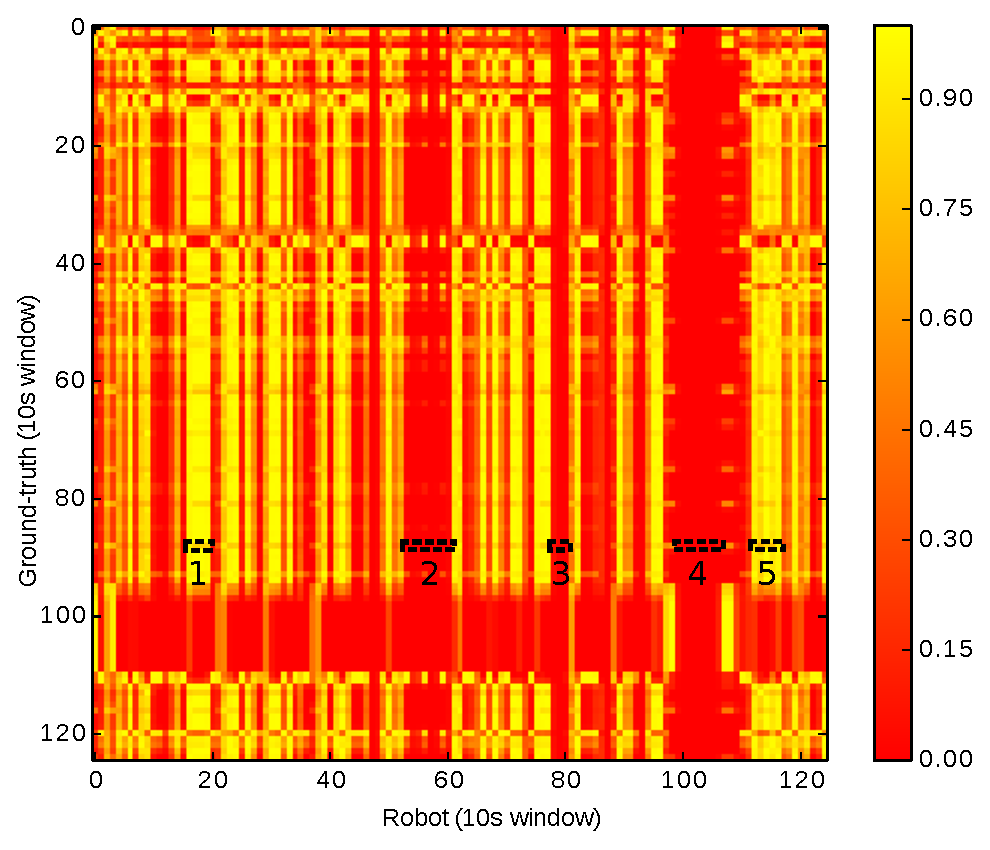
\includegraphics[width=0.8\columnwidth]{bitmap}
    \caption{\small Cosine similarity matrix between real and cap-tured VFOA using a 10 sec. window size computation. The correspondent numbers are shown in figure \ref{fig:realCaptured}.}
    \label{fig:bitmap}
\end{figure}

A relevant trend that can be observed is the continuous `look for approval' situation where the subjects look at the experimenter in order to provide feedback about the robot's response before providing their own one (see yellow boxes in figure \ref{fig:realExpected}). Such transition tablet-experimenter becomes more frequent in several cases, for instance when the experimenter makes a suggestion (orange box in figure \ref{fig:realExpected}), in this case, switch to a more complicated word.

Once the turn-taking is established, a pattern becomes visible during the subject's feedback, when an attempt is performed: Such pattern shows a high intermittent gaze frequency from the tablet to the selection. It also reveals that the subject is using the demonstration model in the selection tablet to provide a better answer to the robot. In fact, subjects decrease the response time after each shift as well as the gaze frequency towards the model suggesting an assimilation over time. Moreover, when a new demonstration is selected for playing, the same behavior is replicated (see yellow boxes in figure \ref{fig:realExpected}).
\\
\subsection{Focus of attention distribution}
Additional information of the head pose can be obtained for the evaluation of the VFOA distribution. Figure \ref{heatmap} show the most salient focuses of attention where the peaks are located. These peaks are mainly projected between the triangle composed by the robot, the writing tablet and the selection tablet using an unsupervised K-means clustering method as figure \ref{kmeans} reveals, considering the observers as negligible.

\begin{figure}[h!]
    \centering
    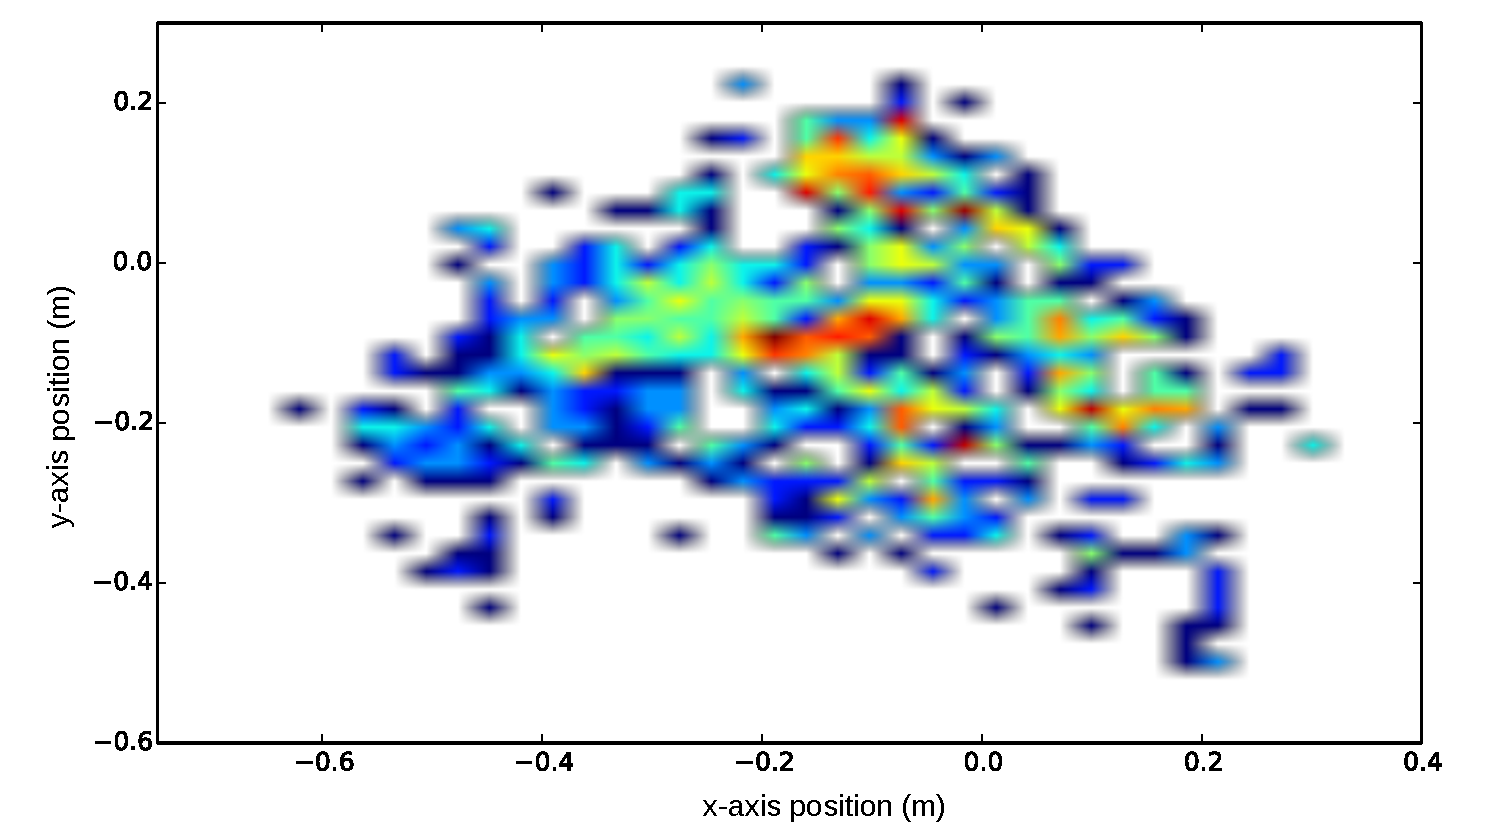
\includegraphics[width=0.9\columnwidth]{heatmap}
    \caption{\small 2D histogram of subject 4 head movements. (head yaw on x-axis, pitch on y-axis). In red, peaks representing the most salient zones.}
    \label{heatmap}
\end{figure}

\begin{figure}[h!]
    \centering
    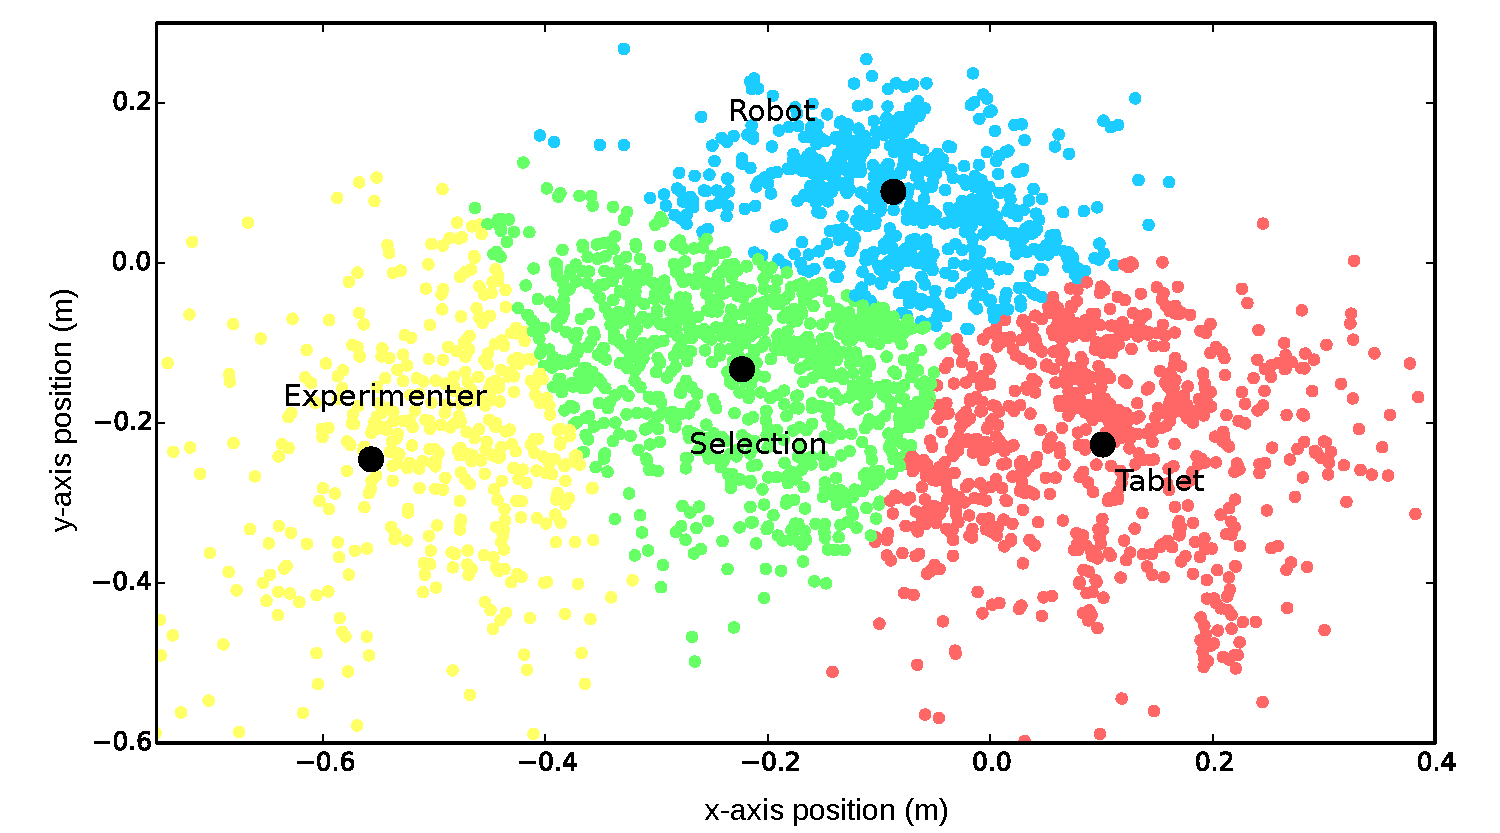
\includegraphics[width=0.9\columnwidth]{kmeans}
    \caption{\small K-means clustering of the head movements.}
    \label{kmeans}
\end{figure}

\subsection{Engagement assessment}
If we consider the case shown in section \ref{fromFaceTo}, evaluating the subject's progression together with the time on task may be an indicator of engagement: If the subject answers so quickly with respect to the previous attempts with a poorer handwriting may be the case she is not engaged anymore. In such hypothetical case an activity switch can be easily implemented in a robot architecture. It confirms the findings reported in \cite{anzalone} where time response to event is proposed to account quality of interaction. 
        
However, a high amount of gaze shift (figure \ref{fig:gazeR}) towards the demonstration provided can reveal that the challenge is too big or no gaze, the exactly the opposite. In this case, the robot response can be adapted to the situation. Similar, but least relevant results are obtained using the correctness (figure \ref{fig:errorR}) of the child's feedback after each attempt. 

\begin{figure}
    \centering
    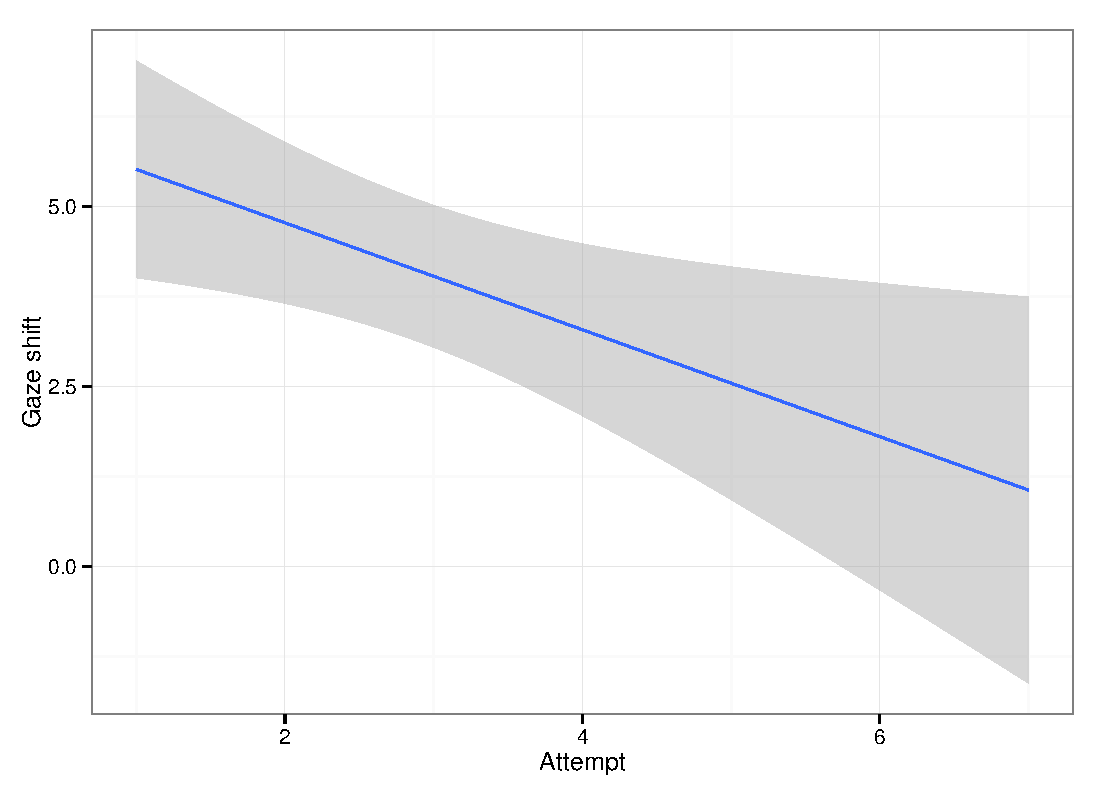
\includegraphics[width=0.9\columnwidth]{gazeR}
    \caption{\small Linear regression of all subject attempts against the occurrences of a gaze shift from the writing tablet towards the model provided. The gray region defines the confidence interval.}
    \label{fig:gazeR}
\end{figure}

\begin{figure}
    \centering
    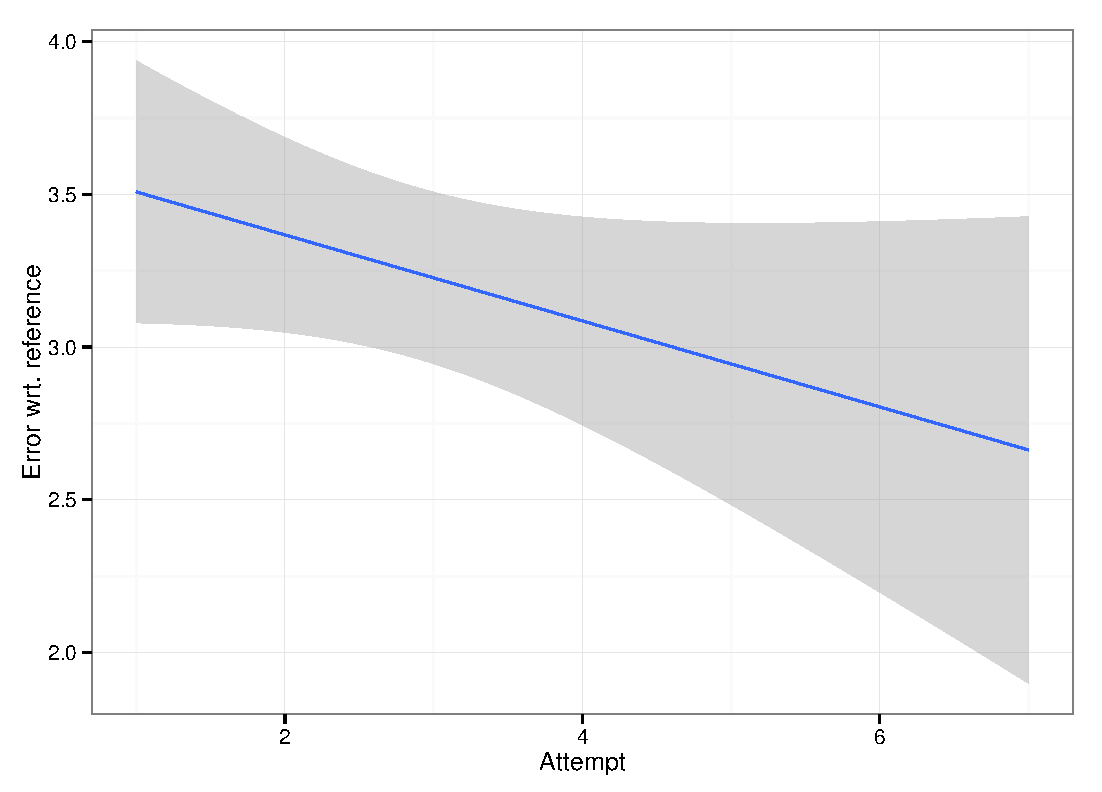
\includegraphics[width=0.9\columnwidth]{errorR}
    \caption{\small Linear regression of all subject attempts against the word correctness, measured as the average euclidean distance of each leter in its corresponding eigenspace with respect to a reference leter. The gray region defines the confidence interval.}
    \label{fig:errorR}
\end{figure}


This information can be used to estimate the child's state during the interaction. For instance, if we consider that a low level of engagement is produced by extremely high or low demanding situations, it is possible to assess the engagement level during the interaction based on gaze shift and word correctness.

It is also important to notice that the initiative of the robot into the learning process in a turn-taking activity produces an effect in the engagement of the human partner. However, experience suggests that a robot that learns evoke a positive action in the partner. But the opposite, a robot that is not able to progress over time, produces the contrary effect.

%Finally, the subjects set their attention more often to the tablet displaying the generated hand-writing during the robot feedback rather than to the robot itself. 


\section{Conclusions}
In this work we have presented an on-line vision-based engagement assessment solution that can be extended to work in different platforms for simulating complex interaction scenarios monitoring several VFOA with a maker-less technology. It provides some benefits like the decrement of the system complexity as well as the increment of the naturalness of the interaction due to the use of an RGB sensor.  

Furthermore, although it has not been tested in a real scenario with several subjects at the same time, the approach also allows to handle such situations too.

During the case study, results show that it is possible to distinguish between long and short feedback episodes based on the gaze shift and depending on the previous attempts performed by the subject. As a result, gaze-shift together with the number of attempts becomes a reliable indicator candidate in the assessment of the engagement during the activity.

Additionally, both the gaze shift and the correctness of the feedback seem to be strictly correlated with the learning gain during the activity as they go in decrement after each attempt provided by the subjects. Despite the fact that these results are encouraging, there is a need of validation with a greater amount of subjects.

Regarding to the approach used, some limitations need to be considered. The most relevant one, the fact that the positions of the VFOA need to be known in advance and defined as static \textit{tf} frames in the system. Moreover, it is important to notice that eye gaze information is neglected which induces a certain amount of error, as well as the noise induced by the 3D pose estimation computed from face landmarkers.

Gaze information acquired during the interactions is not only useful to detect and predict engagement, but also allows the possibility to develop actively the concept gaze-aware robot. In other words, make the system able to estimate where the subject looks at, but also imitate the same subject's VFOA when the activity state allows it. 

%ACKNOWLEDGMENTS are optional
\section*{Acknowledgments}
This research was partially supported by the Funda\c{c}\~{a}o para a Ci\^{e}ncia
e a Tecnologia (FCT) with reference UID/CEC/ 50021/2013, and by the Swiss
National Science Foundation through the National Centre of Competence in
Research Robotics.

\bibliographystyle{abbrv}
\bibliography{sigproc}
\end{document}
